\begin{frame}
    \frametitle{Automatic Story Generation ({\asg})}
    First, why do we care about ASG?
        
    \begin{itemize}[<+(1)->]
        \item Creativity: a long-standing goal of research in AI (at least since the 1950s);
        \item Stories play a central role in human societies;
        \item Cognitive sciences: storytelling-based approaches can be used in communication, education, gaming, marketing, etc.
    \end{itemize}
    
    \uncover<5>{$\hookrightarrow$ \textbf{Can AI help?}}
\end{frame}

\begin{frame}
    \frametitle{Automatic Story Generation ({\asg})}
    {\asg} systems can be divided into three categories \citep{alhussain2021automatic}:
    \begin{enumerate}
        \item \textbf{structural} models, 
        \item \textbf{planning-based} models,
        \item \textbf{machine learning} (ML) models.
    \end{enumerate} 
    \begin{figure}
        \centering
        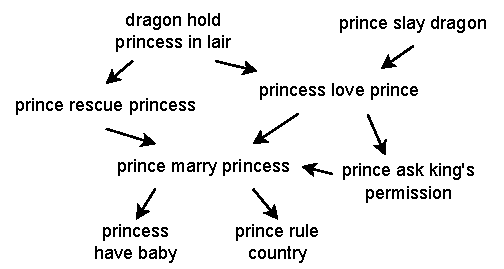
\includegraphics[width=0.5\columnwidth]{pictures/plot_graph.pdf}
        \caption{Plot graph for the sentence: \emph{``the princess loves the prince''} from the planning-based genetic model by \citet{mcintyre2010plot}.}
        \label{fig:plot_graph}
    \end{figure}
\end{frame}

\begin{frame}
    \frametitle{Language Models (LMs)}
    In recent years, \textbf{neural networks} $\to$ heavy dominance of a specific type of ML models: \textbf{language models} (LMs).
    \begin{definition}[Language Model]
        A language model is a \textbf{probability distribution over sequences of tokens}.\\Given a vocabulary $V$ of a set of tokens, a language model $p$ assigns to each sequence of tokens $X = (x_1, \ldots, x_L) \in V^L$ a probability $p(X) \in [0,1].$
    \end{definition}
    \uncover<2>{In this thesis, \textbf{we will only consider language models}.}
\end{frame}

\begin{frame}
    \frametitle{Language Models (LMs)}
    \begin{itemize}[<+->]
        \item Most language models are based on the \textbf{transformer architecture} \citep{vaswani2017attention}.
        \item \textbf{Decoder language models} ({\eg}\ {\gpt}), which use the \emph{decoder} part of the transformer, specialize in text generation.
        \item Most existing \textbf{large language models} ({\llm}s) use a decoder architecture, with some exceptions ({\eg}\ Mamba).
        \item For the definition of {\llm}, we follow \citet{zhao2023survey}: we refer to older transformer-based LMs (\eg\ {\bert}, {\gptt}) as ``pretrained language models'' (PLMs), and ``{\llm}s'' refer to {\gptthree} and more recent models.
        \item The public release of {\chatgpt} (based on {\gptthree}) in late 2022 marked a definite shift in NLP research, namely due to its impressive conversational abilities.
    \end{itemize}
\end{frame}